\section{Demonstration Plan}
\label{sec:demoplan}

%We will launch a spark-shell with InferSpark loaded. Participants to this
%demonstration can try to instantiate, infer and query about three prepared
%models: Latent Dirichlet Allocation (LDA), Sentence-LDA (SLDA), Dirichlet
%Compound Multinomial LDA (DCMLDA). Alternatively, they can define their own
%models in the shell. When InferSpark is instructed to perform inference on a
%model, it can dump the code it generated for participants to browse.
%Participants can also compare the inference performance using InferSpark's
%partition strategy with the generic GraphX partition stratigies. The inference
%runs faster using InferSpark's partition strategy than using GraphX's.

The demonstration will feature several examples of using InferSpark to perform
inference on large clusters and comparisons among InferSpark and other
probabilistic programming frameworks and distributed machine learning
libraries. The examples will be demonstrated via a web-based frontend
connected to a Spark cluster.

\begin{figure}[!h]
    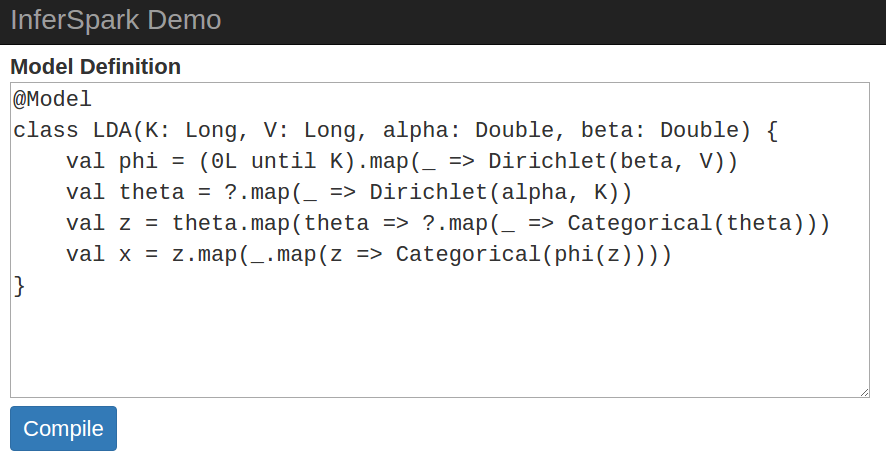
\includegraphics[width=\linewidth]{figs/demo_modeldef.png}
    \vspace*{-10pt}
    \caption{Model Definition}
    \label{fig:demo_modeldef}
\end{figure}

We will prepare a few ready-to-run InferSpark programs for TwoCoin, LDA, 
SLDA \cite{Jo2011}, DCMLDA \cite{Doyle2009} models as well as 
a few datasets loaded to HDFS to run inference on.
The InferSpark programs will show how simply it is to define a model in
InferSpark.  Alternatively, the attendee will be invited to enter their own
model definition in the frontend (see \figref{fig:demo_modeldef}).  The model
will be compiled to byte code and added to the class path when ``Compile''
button is clicked.

%{\bf Eric: please show STEP BY STEP}

%{\bf Eric: now show a screen cap of putting up InferSpark code , .e.,g two coin, on an IDE like Eclipse(?)}


%{\bf: Eric: NOTE that, demo attendance and demo reviewer (including me; I am on VLDB demo committee) perhaps to see *G*raphical UI, i.e., button click, toolbar)  please turn your 'console' base screen capture to UI base screen capture; that substainatilly increase the chance!}

\begin{figure}[!h]
    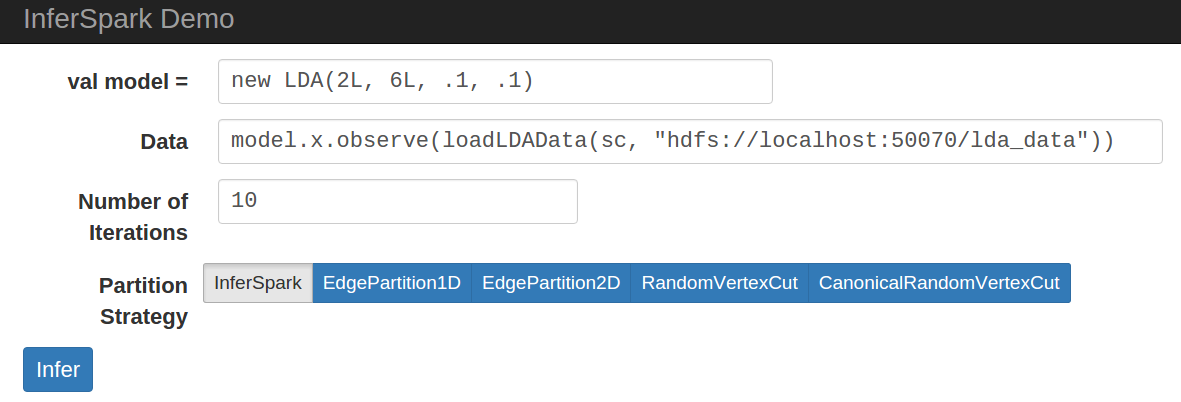
\includegraphics[width=\linewidth]{figs/demo_param.png}
    \vspace*{-10pt}
    \caption{Setting parameters and observed variables}
    \label{fig:demo_param}
\end{figure}

Attendee will be allowed to change some inference options such as dataset, the
number of iterations and the edge partition strategy in the parameter settings
page (\figref{fig:demo_param}). In the figure, the hyperparameters of the LDA
model $\alpha$ and $\beta$ are both set to $0.1$. The vocabulary size is 6 and
the number of topics is 2. The dataset to run inference on is a synthetic data
set which contains a few simple sentences describing sports or food. The
inference will be run for 10 iterations. The edge partition strategy is set to
the InferSpark default. The inference will be launched when ``infer'' is
clicked.

\begin{figure}[!h]
    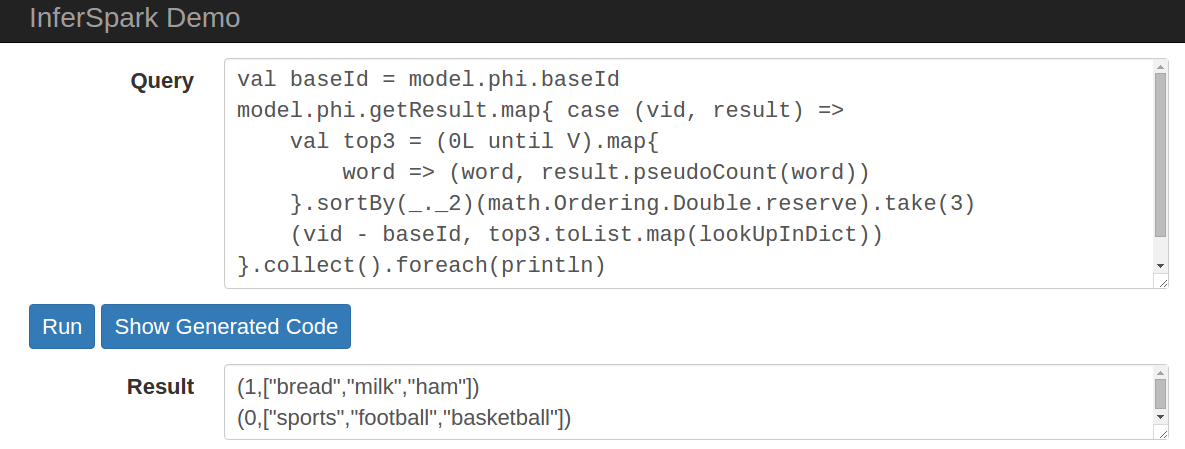
\includegraphics[width=\linewidth]{figs/demo_get_result.png}
    \vspace*{-10pt}
    \caption{Query posterior distribution}
    \label{fig:demo_get_result}
\end{figure}

After the inference is completed, attendee will be shown a result querying
page (see \figref{fig:demo_get_result}). The posterior distribution of the
random variable in the model can be acquired by calling ``getResult'' API on
the random variable. In the example shown in \figref{fig:demo_get_result}, top
3 most probable words are shown for each topic.  The attendee can also browse
the generated inference code by clicking ``Show Generated Code'' button.

%{\bf Eric: really don't understand your Figure 7; make the output less 'developer' feel, but more your mummy's feel, remove all those 11:1313 INFO....}

Finally, we will set up other probabilistic programming frameworks, e.g.,
Infer.NET. We will provide the program in those frameworks that
implement the same models. Attendee will see how much 
simpler and more efficient it is to
run inference on large scale data using InferSpark than other frameworks.

To demonstrate the benefit of using InferSpark's optimized partition strategy,
attendee will be invited to set the partition strategy to the GraphX's
built-in ones when the same inference tasks are run. With the built-in edge
partition strategies, Spark may be slowed down due to imbalance of partitions
or even crash due to block size limits. InferSpark's partition strategy,
in contrast, will help balance the load and thus shorten the inference time.

